\documentclass{article}
\usepackage{hyperref}
\usepackage{graphicx} % Required for inserting images

\title{MVP}
\author{Automatic Project Detection And Tooling For Devs}
\date{}

\begin{document}
\maketitle

\section{User stories}

\begin{figure}[h]
    \centering
    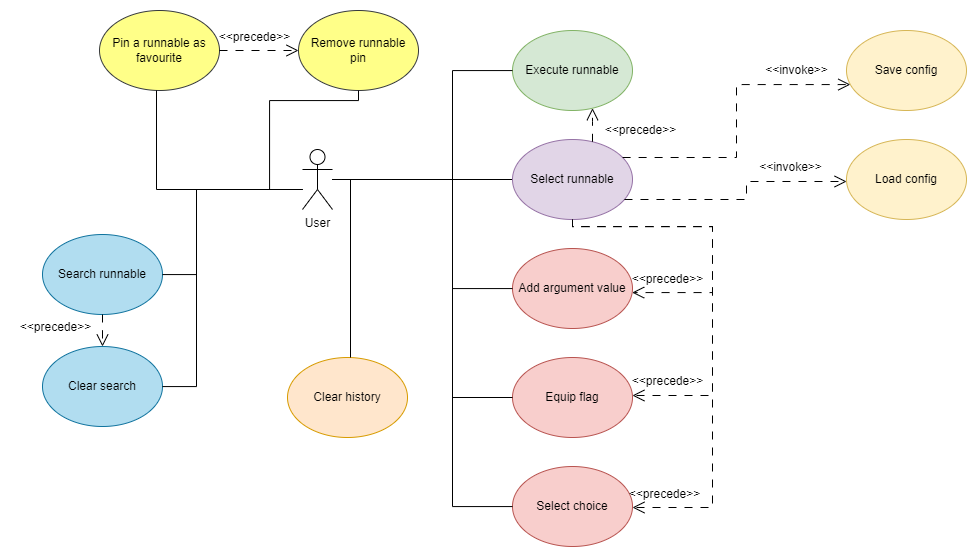
\includegraphics[width=1\linewidth]{img/use_case_diagram.drawio.png}
    \caption{Use case diagram}
    \label{fig:enter-label}
\end{figure}

\subsection{Select executable}
\begin{itemize}
    \item \textbf{As a} user \textbf{I want} to select an executable or a script from the list of programs that the app found, \textbf{so that} I can configure its arguments.
\end{itemize}

\subsection{Add value to argument}
\begin{itemize}
    \item \textbf{As a} user \textbf{I want} to give a value to an argument \textbf{so that} I can add it to the configuration.
\end{itemize}

\subsection{Toggle flag}
\begin{itemize}
    \item \textbf{As a} user \textbf{I want} set a flag \textbf{so that} I can chose that the flag stores True or False.
\end{itemize}

\subsection{Select choices}
\begin{itemize}
    \item \textbf{As a} user \textbf{I want} to choose a value from the list of possible choices for the argument \textbf{so that} I can set it.
\end{itemize}

\subsection{Execute programs}
\begin{itemize}
    \item \textbf{As a} user \textbf{I want} to execute a configured program \textbf{so that} I can press a button on the screen and the tool runs it with the given arguments.
\end{itemize}

\subsection{Save config}
\begin{itemize}
    \item \textbf{As a} user \textbf{I want} to save the configuration that I gave before \textbf{so that} the program saves it for me.
\end{itemize}

\subsection{Load config}
\begin{itemize}
    \item \textbf{As a} user \textbf{I want} to load the previously saved configuration \textbf{so that} the program loads it for me.
\end{itemize}

\subsection{Clear history}
\begin{itemize}
    \item \textbf{As a} user \textbf{I want} to clear my configuration history \textbf{so that} the program deletes every configuration.
\end{itemize}

\subsection{Pin an executable}
\begin{itemize}
    \item \textbf{As a} user \textbf{I want} to pin an executable or script \textbf{so that} the program highlights it.
\end{itemize}

\subsection{Unpin an executable}
\begin{itemize}
    \item \textbf{As a} user \textbf{I want} unpin an executable \textbf{so that} the program removes the highlight.
\end{itemize}

\subsection{Search executable}
\begin{itemize}
    \item \textbf{As a} user \textbf{I want} find a specified program \textbf{so that} I can search it from the list.
\end{itemize}

\subsection{Clear search}
\begin{itemize}
    \item \textbf{As a} user \textbf{I want} to clear the search history \textbf{so that} the program doesn't show in the list of previously searched items.
\end{itemize}

\section{Prioritized user stories}

Prioritizing with the help of MoSCoW method.
\begin{itemize}
    \item M - Must have
    \item S - Should have
    \item C - Could have
    \item W - Won't have
\end{itemize}

\subsection{Must have user stories:}
\begin{itemize}
    \item Select executable:
    \begin{itemize}
        \item Filters all executables from the working direcoty.
        \item Collects all details of these, such as description, name, and arguments. It also collects all information about the arguments.
        \item Full path to the program, that will be needed during execution.
    \end{itemize}
    \item Execute program:
    \begin{itemize}
        \item Executing the programs with using its full path and the appropriate compiler or interpreter.
        \item If information available of the values of the arguments, These must be used during execution.
    \end{itemize}
    \item Add argument
    \begin{itemize}
        \item This user story ensures that the user can provide a value for an argument as input.
    \end{itemize}
\end{itemize}

\subsection{Should have user stories}
\begin{itemize}
    \item Toggle flag
    \begin{itemize}
        \item If the argument is a flag, user can switch whether it should store a true or false.
    \end{itemize}
    \item Select choices
    \begin{itemize}
        \item If there are choices within the argument, the user should select one of them.
    \end{itemize}
    \item Save config
     \begin{itemize}
         \item Users are able to store their configurations.
     \end{itemize}
     \item Load config
     \begin{itemize}
         \item Users are able to load their previously saved configurations.
     \end{itemize}
     \item Clear history
     \begin{itemize}
         \item Users are able to delete their configurations.
     \end{itemize}
\end{itemize}

\subsection{Could have user stories}
\begin{itemize}
    \item Search an executable
    \begin{itemize}
        \item Users are able to search for specified scripts.
    \end{itemize}
    \item Clear search
    \begin{itemize}
        \item After searching users can delete their search history.
    \end{itemize}
\end{itemize}

\subsection{Won't have user stories }
\begin{itemize}
    \item Pin an executable
    \begin{itemize}
        \item Users are able to pin programs as favourite, and those will be highlighted.
    \end{itemize}
    \item Unpin an executable
    \begin{itemize}
        \item Users are able to unpin a pinned program.
    \end{itemize}
\end{itemize}

\section{The content of the MVP}
MVP should contain these user stories, which have been prioritized.
\begin{itemize}
    \item Select executable
    \item Add values to arguments
    \item Toggle flag
    \item Select choices
    \item Execute program
    \item Save config
    \item Load config
    \item Clear history
    \item Search executable
    \item Clear search
\end{itemize}

\section{MVP complete}
The complete MVP should contain these user stories below.
\begin{itemize}
    \item Select executable
    \item Add values to arguments
    \item Toggle flag
    \item Select choices
    \item Execute executable
    \item Save config
    \item Load config
    \item Clear history
\end{itemize}

\section{MVP minimal}
None of this user stories can be taken out to avoid losing the point of MVP.
\begin{itemize}
    \item Select executable
    \item Add values to arguments
    \item Execute programs
\end{itemize}

\section{MVP real}
The user stories below have the potential to be implemented realistically by the end of the project.
\begin{itemize}
    \item Select executable
    \item Add argument value
    \item Toggle flag
    \item Select choices
    \item Execute program
\end{itemize}

\section{KPI deffinition}

\section{KPI goal}

\end{document}
